\documentclass{beamer}
\usetheme{Copenhagen}
\usepackage[utf8]{inputenc}

\title{Tutorial VS Code, bash y github}
\author{\texorpdfstring{Author\newline\url{www.github.com/mlacosta}}{Author}}
\author{Ing. Mariano L. Acosta}
\logo{
\includegraphics[width=.1\textwidth]{img/logo.jpg}}

\begin{document}
\begin{frame}[plain]
    \maketitle
    	\begin{center}
    		
\includegraphics[scale=.025]{img/icons/linkedin.png}{ \tiny linkedin.com/mlacosta} \\
    		
\includegraphics[scale=.02]{img/icons/github.png}{ \tiny github.com/mlacosta} \\
    		
\includegraphics[scale=.006]{img/icons/twitch.png}{ \tiny twitch.tv/mariandevs} \\
    		\vspace{.5cm}
    		\textbf{Tiempo de Exposición:}{ 1 hora}\\
    		\vspace{.2cm}
    		
\includegraphics[scale=.15]{img/banner.JPG} 
    	\end{center}
    	

    
\end{frame}


\begin{frame}
	\frametitle{Objetivos}
		\textbf{Presentación de herramientas necesarias para el desarrollo: }
			\vspace{.3cm}
		\begin{itemize}
			\item Ver VS Code y sus extensiones
			\vspace{.3cm}
			\item Aprender a usar el CLI y sus comandos básicos
			\vspace{.3cm}
			\item Entender qué es GIT y cómo usarlo
			\vspace{.3cm}
			\item Aprender a usar repositorios en Github
			\vspace{.3cm}
		\end{itemize}
\end{frame}


\section{Presentación de Herramientas}

\begin{frame}{Visual Studio Code}
	\begin{columns}
  		\begin{column}{.5\textwidth}
			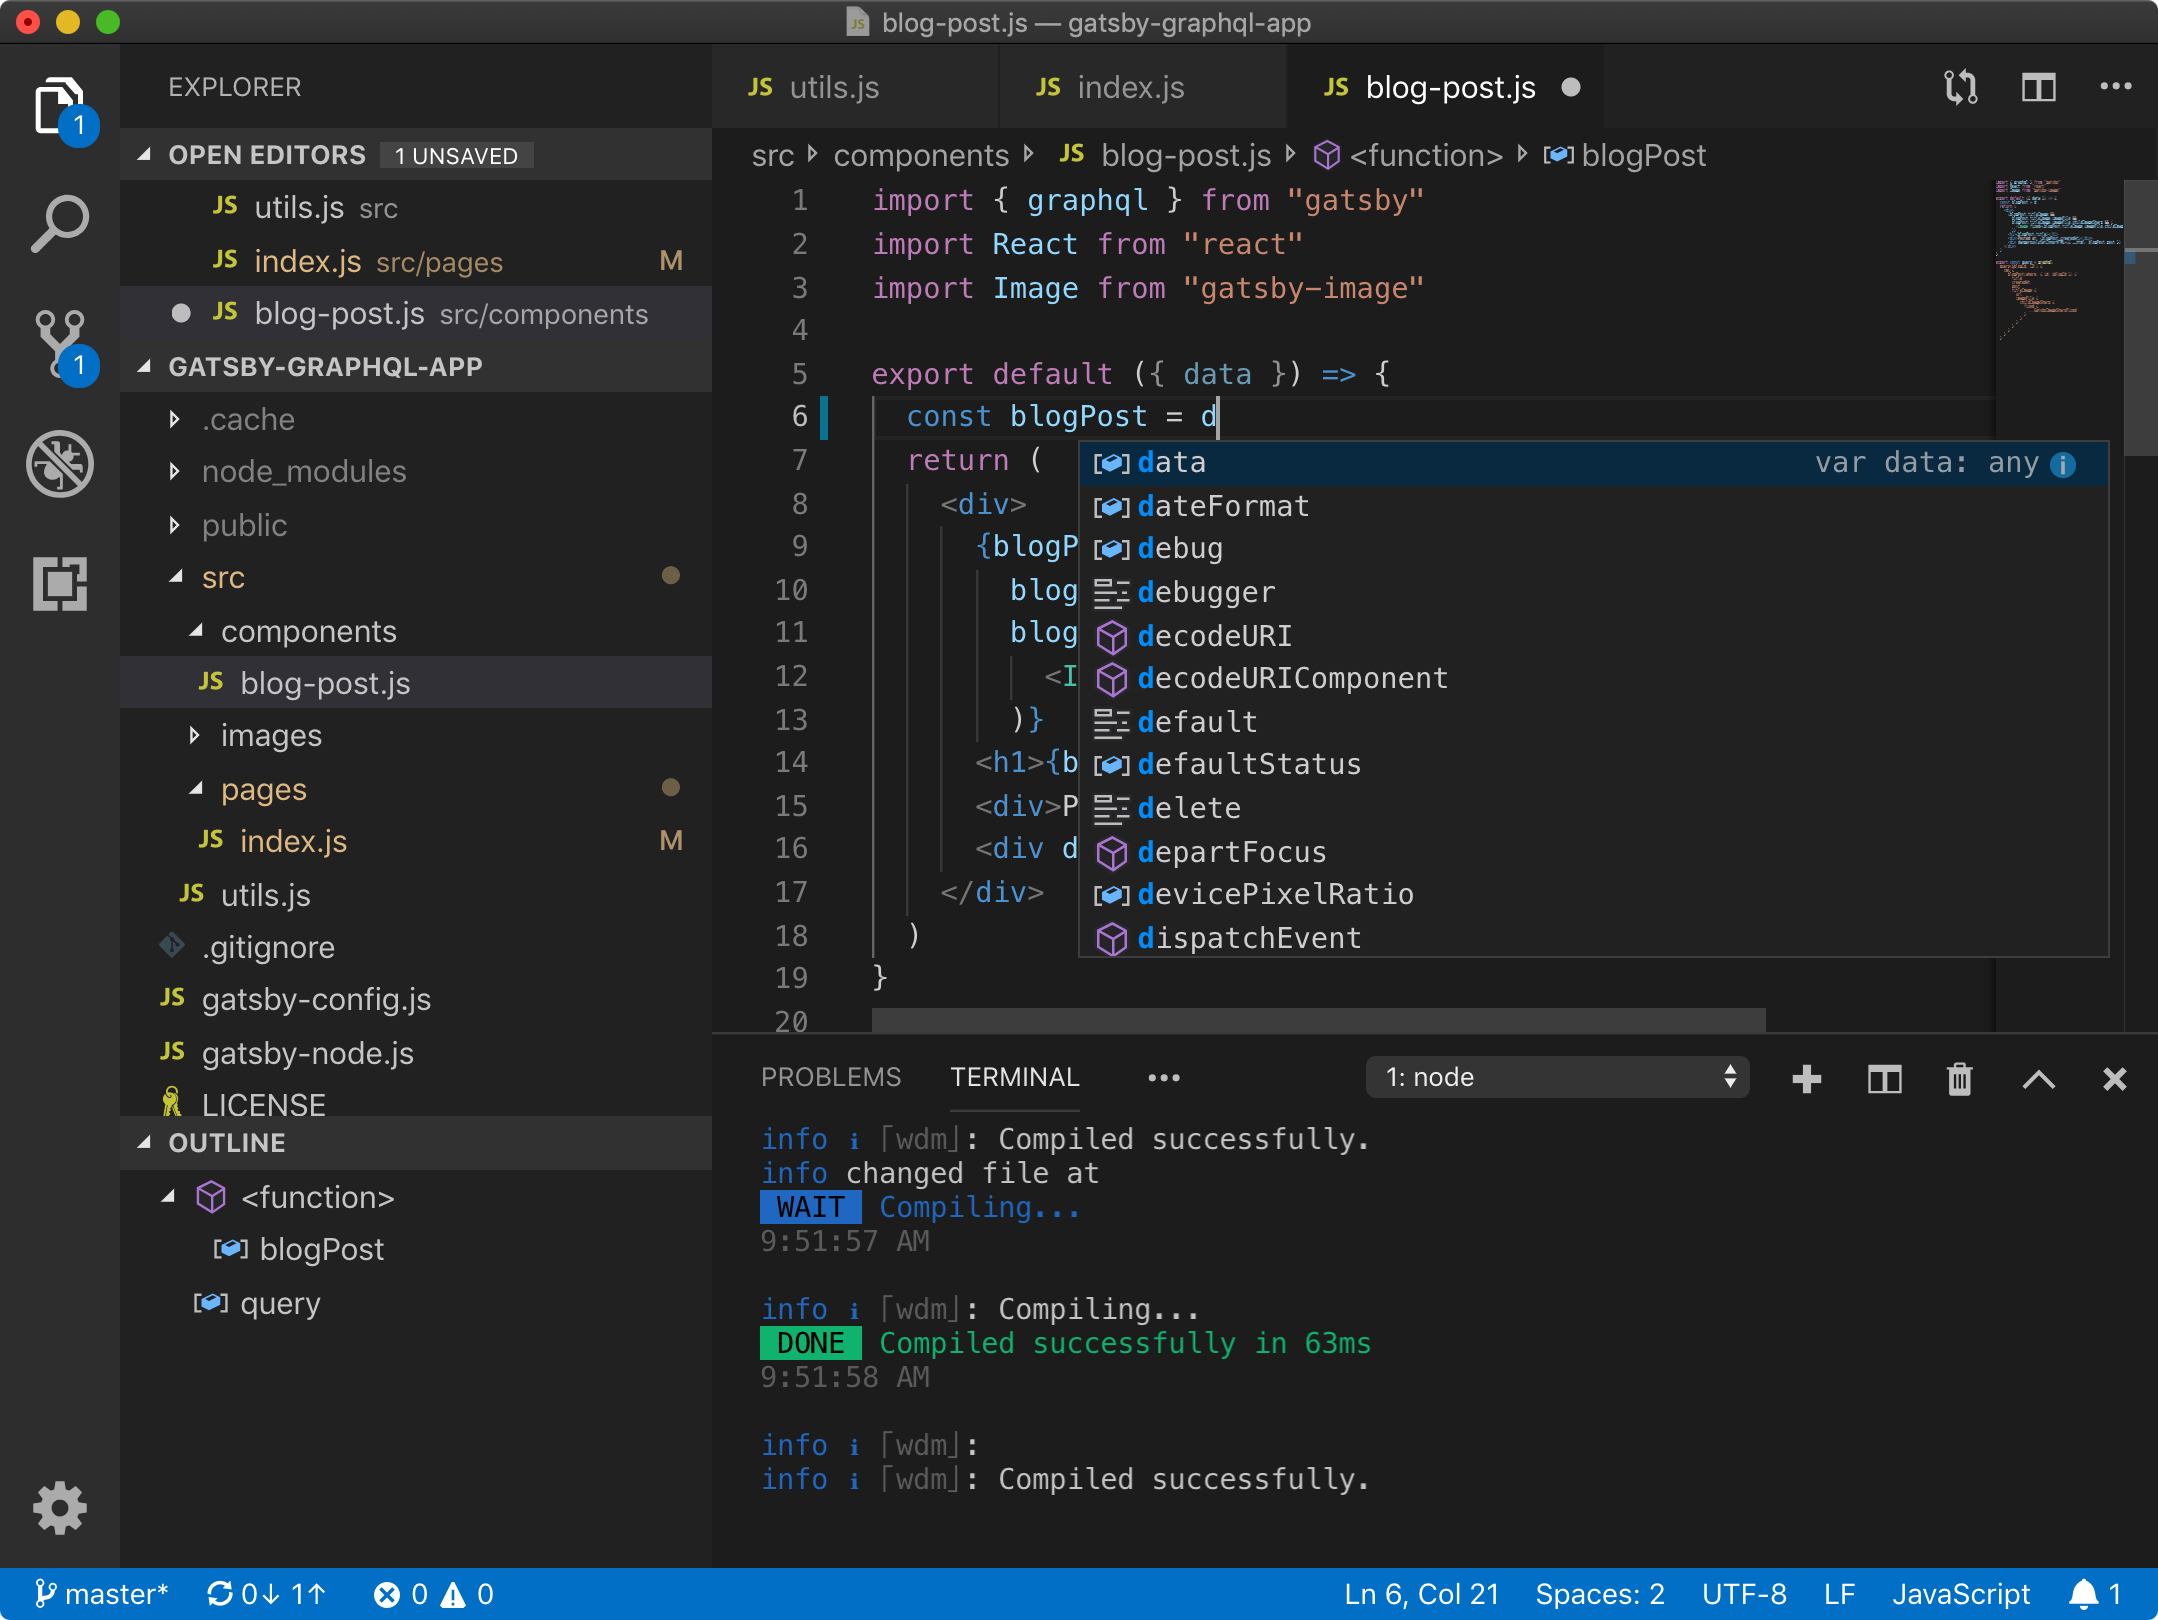
\includegraphics[scale=.15]{img/vscode.png}
		\end{column}
		\begin{column}{.5\textwidth}
				
			\begin{itemize}
				\item IntelliSense (autocompletado de código, info extra, etc.)
				\item Altamente customizable (plugins/temas)
				\item Prestaciones optimizadas para desarrollo web
				\item Integración con JSX/React, HTML, CSS, JSON, etc...
			\end{itemize}
		\end{column}
	\end{columns}
\end{frame}

\begin{frame}{Bash Shell (Windows)}
	\begin{columns}
		\begin{column}{.5\textwidth}
			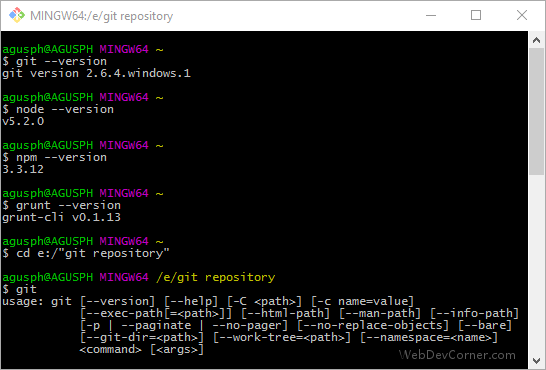
\includegraphics[scale=.3]{img/git_bash.png}
		\end{column}
		\begin{column}{.5\textwidth}
			
			\begin{itemize}
				\item Emulación de la linea de comandos de UNIX
				\item Amigable para principiantes y expertos
				\item Automatización de tareas repetitivas (scripts)
				\item Soporte de la comunidad (recursos disponibles)
			\end{itemize}
		\end{column}
	\end{columns}
	
\end{frame}

\begin{frame}{Git | Control de Versiones}
	\begin{columns}
		\begin{column}{.3\textwidth}
			
\includegraphics[scale=.1]{img/git_logo.png}
		\end{column}
		\begin{column}{.6\textwidth}
			
			\begin{itemize}
				\item Creado por Linus Torvalds en 2005 (Linux)
				\item Registros de todos los cambios en el código (undoing)
				\item Colaboración con múltiples desarrolladores (branching)
				\item Prototipado/Desarrollo de prestaciones (features)
			\end{itemize}
		\end{column}
	\end{columns}
\end{frame}

\begin{frame}{Git | Control de Versiones}

	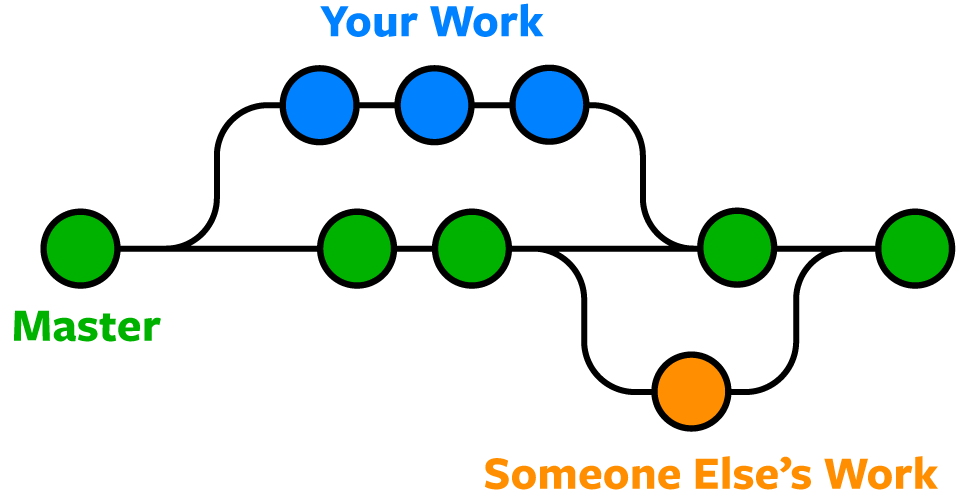
\includegraphics[scale=.3]{img/branches.png}
	
\end{frame}

\begin{frame}{Git | Control de Versiones}
	
	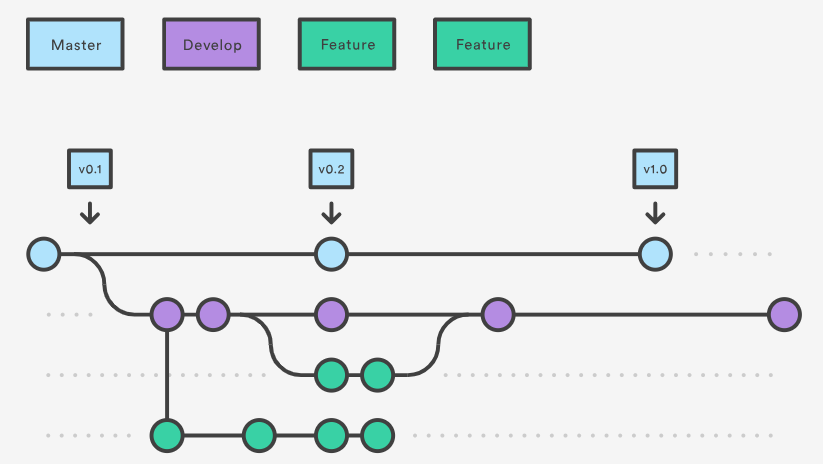
\includegraphics[scale=.35]{img/git_project.png}
	
\end{frame}

\begin{frame}{Github}
	\begin{columns}
		\begin{column}{.4\textwidth}
			
\includegraphics[scale=.1]{img/github.jpeg}
		\end{column}
		\begin{column}{.75\textwidth}
			
			\begin{itemize}
				\item Servicio para almacenar y compartir código 
				\vspace{0.25cm}
				\item Colaboración en proyectos Open Source
				\vspace{0.25cm}
				\item Creación de portfolio personal
				\vspace{0.25cm}
				\item Gran cantidad de software listo para descargar (ver licencias)
				\vspace{0.25cm}
				\item Existen otras alternativas (Bitbucket, SourceForge, etc...)
			\end{itemize}
		\end{column}
	\end{columns}
	
\end{frame}


\section{Comandos de Consola (Bash)}


\begin{frame}
	
	\textbf{Comandos}
	\begin{block}{\textbf{Cambiar Directorio cd}}
		Moverse en el sistema de archivos. 
		Sus parámetros pueden ser un directorio, subdirectorio o directorio padre\\
	\end{block}	
	\begin{center}
		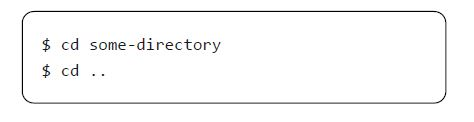
\includegraphics[scale=.6]{img/bash/cd.JPG}
	\end{center}
	
\end{frame}

\begin{frame}
	
	\textbf{Comandos}
	\begin{block}{\textbf{Crear Directorio mkdir}}
		Crear directorio de acuerdo a su argumento. Puede darse un path o un nombre.
	\end{block}	
	\begin{center}
		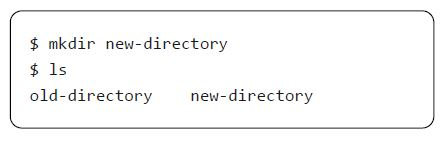
\includegraphics[scale=.6]{img/bash/mkdir.JPG}
	\end{center}
	
\end{frame}

\begin{frame}

	\textbf{Comandos}
	\begin{block}{\textbf{Crear archivo touch}}
		Crea un nuevo archivo bajo el directorio con el nombre y extensión provistas
	\end{block}	
	\begin{center}
		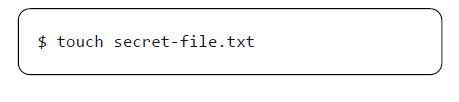
\includegraphics[scale=.6]{img/bash/touch.JPG}
	\end{center}

\end{frame}

\begin{frame}
	
	\textbf{Comandos}
	\begin{block}{\textbf{List ls}}
		Mostrar los contenidos del directorio
	\end{block}	
	\begin{center}
		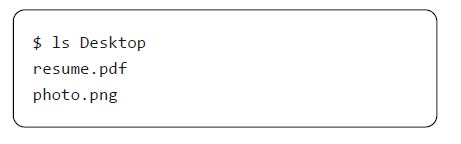
\includegraphics[scale=.6]{img/bash/ls.JPG}
	\end{center}
	
\end{frame}

\begin{frame}
	
	\textbf{Comandos}
	\begin{block}{\textbf{ls opciones}}
				\begin{itemize}
			\item ls -a: mostrar archivos ocultos
			\item ls -l: mostrar formato largo
			\item ls -t: mostrar fecha de modificación
		\end{itemize}
	\end{block}	
	\begin{center}
		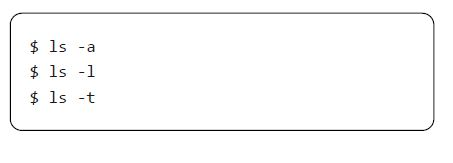
\includegraphics[scale=.6]{img/bash/ls2.JPG}
	\end{center}
	
\end{frame}

\begin{frame}
	
	\textbf{Comandos}
	\begin{block}{\textbf{Copiar cp}}
		Copiar archivos o directorios. \\ 
		La estructura básica es \$ cp [fuente] [destino]
	\end{block}	
	\begin{center}
		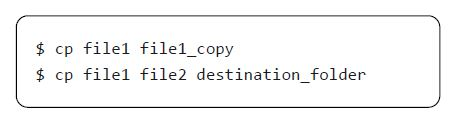
\includegraphics[scale=.6]{img/bash/cp.JPG}
	\end{center}
	
\end{frame}

\begin{frame}
	
	\textbf{Comandos}
	\begin{block}{\textbf{Mover mv}}
		Mover archivos dentro de directorios. \\ 
		La estructura básica es \$ mv [nombre\_archivo] [destino]
	\end{block}	
	\begin{center}
		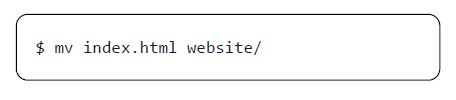
\includegraphics[scale=.6]{img/bash/mv.JPG}
	\end{center}
	
\end{frame}

\begin{frame}
	
	\textbf{Comandos}
	\begin{block}{\textbf{Borrar rm}}
		Eliminar archivos y/o directorios. \\ 
		El flag -r remueve directorios y todo su contenido\\
		La estructura básica es \$ rm -r [nombre\_recurso] 
	\end{block}	
	\begin{center}
		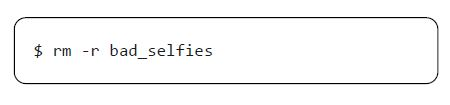
\includegraphics[scale=.6]{img/bash/rm.JPG}
	\end{center}
	
\end{frame}

\begin{frame}
	
	\textbf{Comandos (Avanzados)}
	\begin{block}{\hyperlink{https://mywiki.wooledge.org/BashGuide/InputAndOutput}{https://mywiki.wooledge.org/BashGuide/InputAndOutput}}
		Redireccionar  \\
		\vspace{0.3cm}
		Mostrar contenido \\ 
		\vspace{0.3cm}
		Transferencia \\
		\vspace{0.3cm}
		Buscar \\
	\end{block}	

\end{frame}

\begin{frame}
	
	\textbf{Comandos (Scripts)}
	\begin{block}{https://devhints.io/bash}
		- Automatizar tareas de programación, como crear directorios y archivos, búsqueda de datos, generar repositorios, etc...\\
		\vspace{0.3cm}
		- Creación de Aliases
	\end{block}	
	
\end{frame}


\section{Visual Code Studio}
	\begin{frame}
		
		\begin{block}{\textbf{Demostración VS Code + Bash}}
			- Creación de un sistema de archivos \\
			\vspace{0.3cm}
			- Comando 'code' \\
			\vspace{0.3cm}
			- Ejemplo de Aliases y Scripts \\
			\vspace{0.3cm}
			- Terminal Integrado \\
			\vspace{0.3cm}
			- Autocompletado de Código \\
		\end{block}	
		
	\end{frame}

	\begin{frame}
		\textbf{Plugins - Extensiones para VS Code (Ctrl + shift + p)}
		\begin{center}
			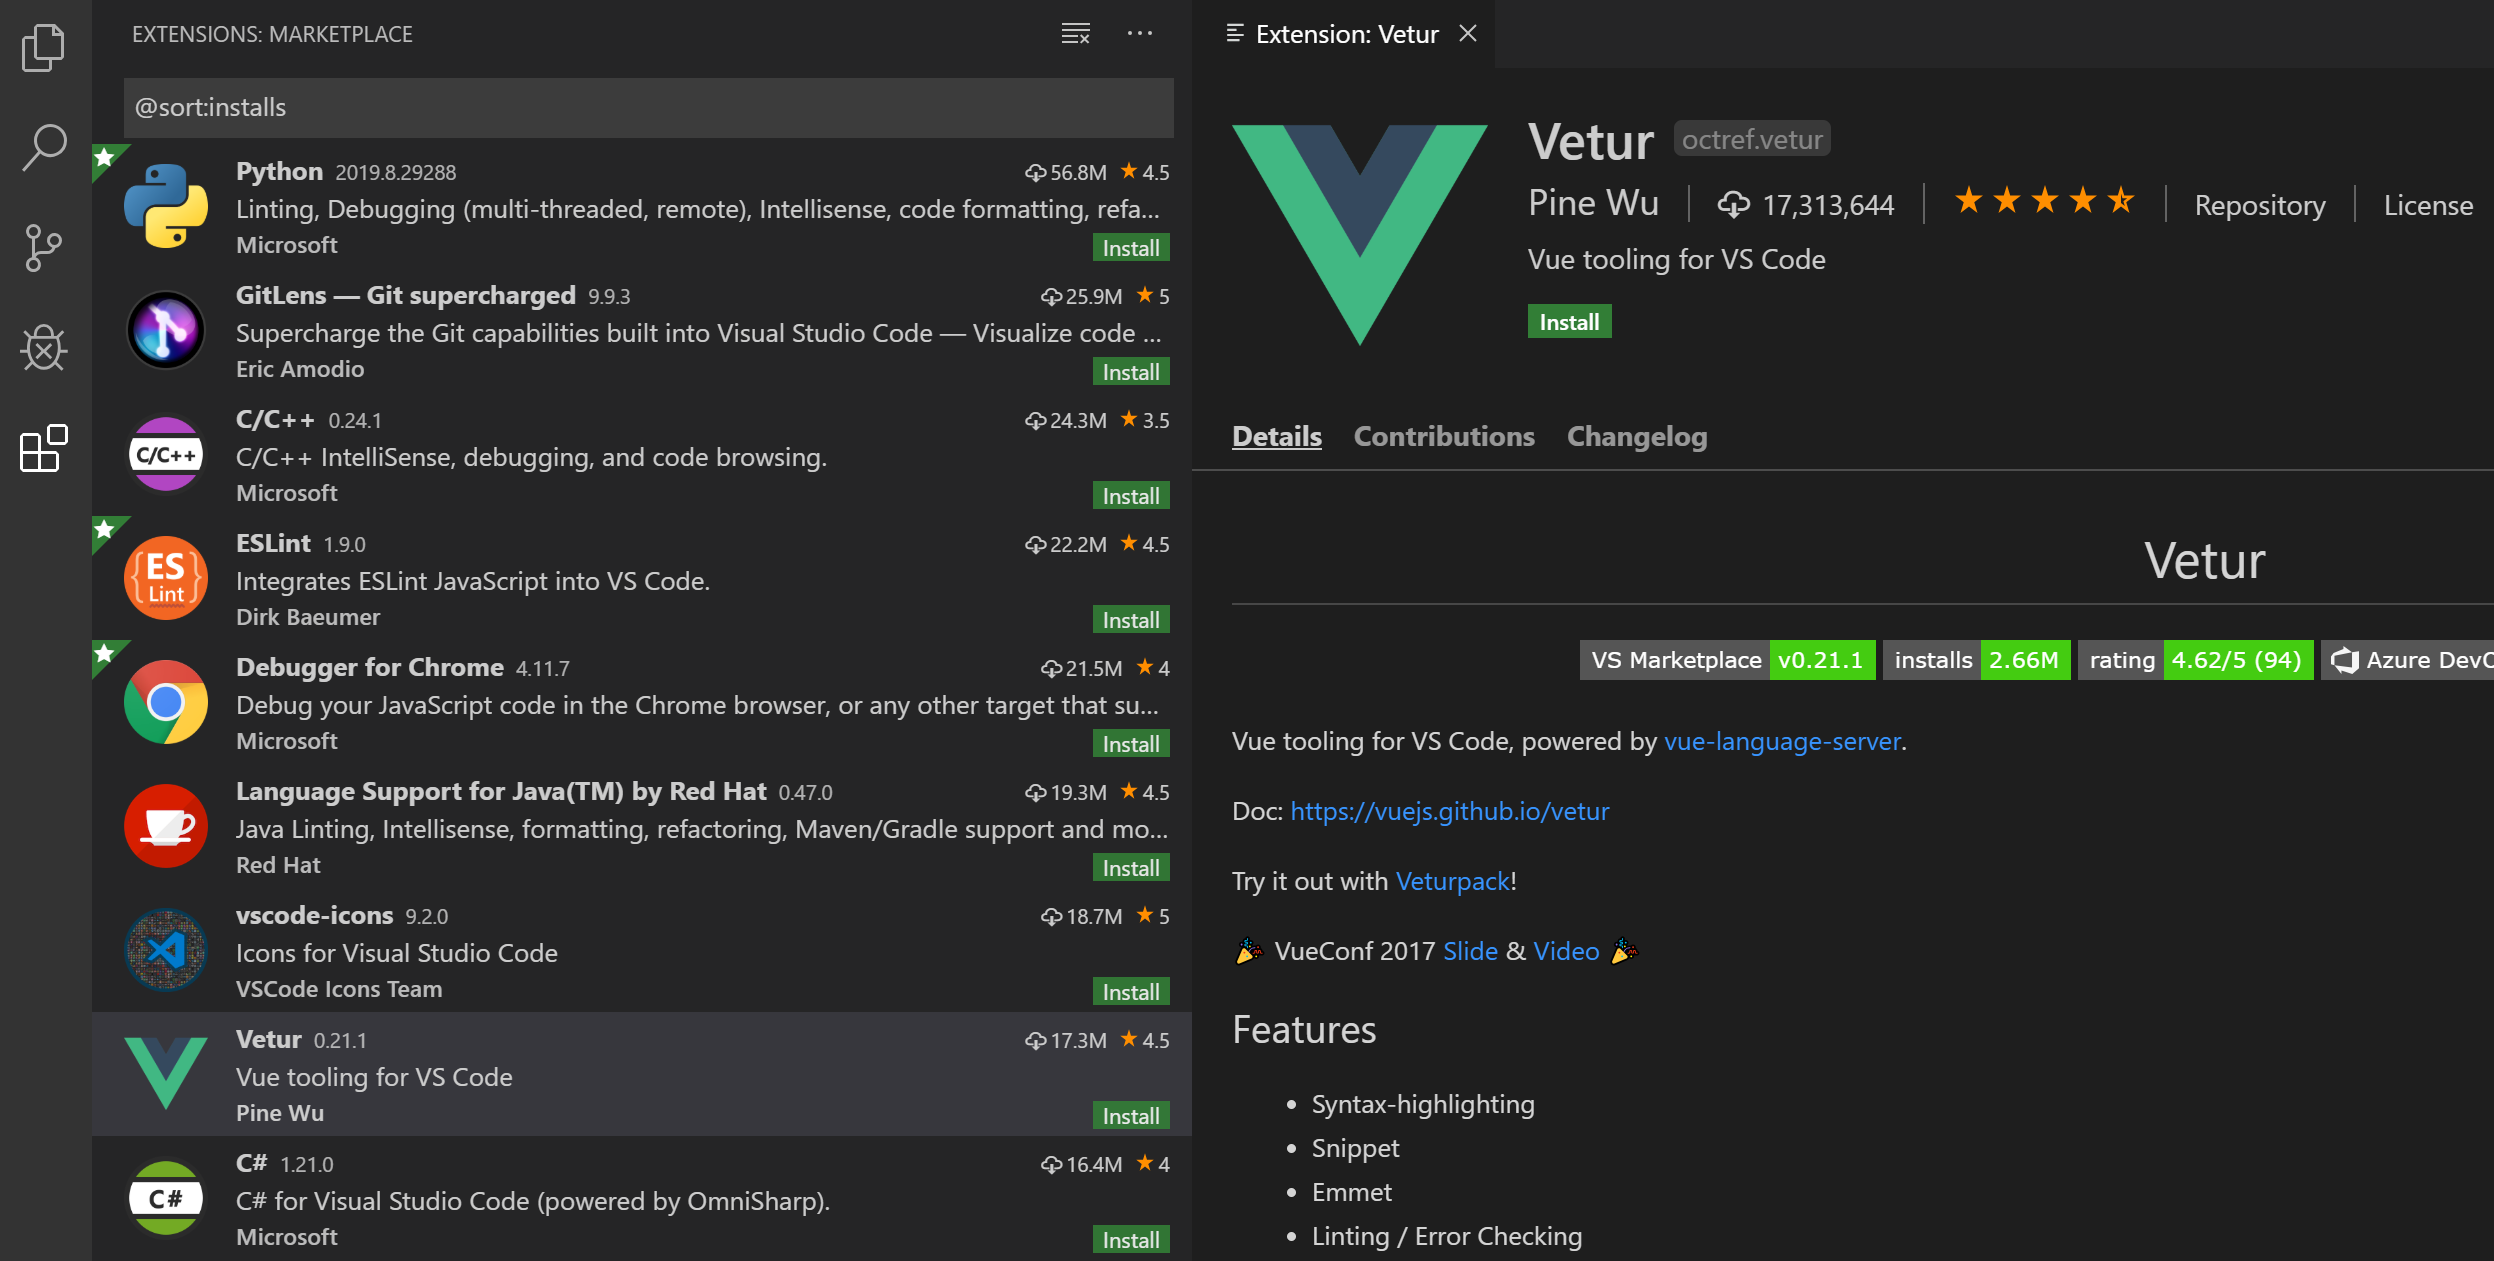
\includegraphics[scale=.3]{img/extensions.png}
		\end{center}
	\end{frame}

\section{Comandos de Git}
	\begin{frame}
		\begin{center}
			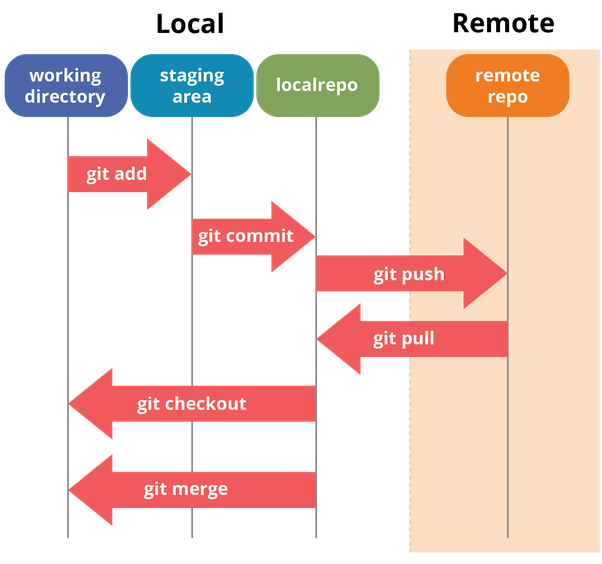
\includegraphics[scale=.3]{img/git_diagram.png}
		\end{center}
	\end{frame}
	\begin{frame}
	Se debe inicializar GIT en el directorio raiz del proyecto y procurar \textbf{NO} volver a hacerlo en ningún subdirectorio del mismo. 
		\begin{block}{\textbf{Creación de un repositorio local}}
			\$ git init\\
			\vspace{0.3cm}
			\$ git add nombre\_archivo ó \$ git add .\\
			\vspace{0.3cm}
			\$ git commit -m "mi primer commit" \\
			\vspace{0.3cm}
		\end{block}	
	\end{frame}

	\begin{frame}
	\textbf{DEMOSTRACIÓN}\\ Luego crean un Repo en github y lo sincronizan así:
		\begin{block}{\textbf{Agregar repositorio remoto}}
			\small \$ git remote add origin https://github.com/tu\_usuario/nombre\_repo.git\\
			\vspace{0.3cm}
			\small \$ git branch -M main\\
			\vspace{0.3cm}
			\small \$ git push -u origin main \\
			\vspace{0.3cm}
		\end{block}	
	\end{frame}


	\begin{frame}
		\textbf{La primera vez que quieran hacer un push a su cuenta con el CLI les van a pedir que ingresen usuario y contraseña} \\
		\vspace{1cm}
		\textbf{Formas de Autenticación}
		\begin{itemize}
			\item HTTPS (Recomendado/Fácil) (user/password)
			\item SSH (Más complicado/Más seguro) (clave privada)
		\end{itemize}
	\end{frame}

	\begin{frame}
		\textbf{DEMOSTRACIÓN} Cada vez que hagan cambios locales y quieran actualizar el repo:
		\begin{block}{\textbf{Actualizar repositorio remoto}}
			\small \$ git add . \\
			\vspace{0.3cm}
			\small \$ git commit -m "algun comentario relacionado"\\
			\vspace{0.3cm}
			\small \$ git push \\
			\vspace{0.3cm}
			\textbf{Alternativamente:}\\
			\vspace{0.3cm}
			\small \$ git commit -a -m "algun comentario relacionado"\\
			\vspace{0.3cm}
			\small \$ git push \\
			\vspace{0.3cm}
		\end{block}	
	\end{frame}

	\begin{frame}
		\textbf{DEMOSTRACIÓN} 
		\begin{block}{\textbf{¿Qué pasa si modifiqué el repo en github y quiero bajar los cambios a mi PC?}}
			\vspace{0.3cm}
			\small \$ git fetch \\
			\vspace{0.3cm}
			\small \$ git merge origin/main\\
			\vspace{0.3cm}
			\textbf{Alternativamente:}\\
			\vspace{0.3cm}
			\small \$ git pull
			\vspace{0.3cm}
		\end{block}	
	\end{frame}

	\begin{frame}
		\textbf{DEMOSTRACIÓN} 
		\begin{block}{\textbf{Más Comandos}}
			\vspace{0.3cm}
			 \$ git status   \small -Ver archivos modificados y sin trackear- \\
			\vspace{0.3cm}
			 \$ git log    \small -Ver historial de commits (apretar 'q' para salir)-\\
			\vspace{0.3cm}
		    \$ git diff nombre\_archivo    \small -Ver cambios en el código-\\
			\vspace{0.3cm}
		\end{block}	
	\end{frame}

	\begin{frame}
	\textbf{DEMOSTRACIÓN} 
		\begin{block}{\textbf{Más Comandos}}
			\vspace{0.3cm}
			\small \$ git reset HEAD nombre\_archivo   \tiny -Remover todos los archivos del staging- \\
			\vspace{0.3cm}
			\small \$ git checkout -- nombre\_archivo \tiny -Revertir el estado de un archivo antes de cambiarlo-\\
			\vspace{0.3cm}
			\small \$ git rm -r nombre\_dir   \tiny -Eliminar archivo/directorio del disco y del repo local-\\
			\vspace{0.3cm}
			\small \$ git rm nombre\_archivo --cache   \tiny -Eliminar archivo \textbf{sólo} del repo local-\\
			\vspace{0.3cm}
		\end{block}	
	\end{frame}

	\begin{frame}{.gitignore}
		\textbf{DEMOSTRACIÓN} \\
		\vspace{.5cm}
		Muchas veces no es necesario o no queremos agregar archivos/carpetas a un repositorio, para ello nos servimos del archivo .gitignore
	\end{frame}

	\begin{frame}
		\textbf{Para aprender más sobre GIT:} \\
		\vspace{1cm}
		\begin{center}
			https://www.atlassian.com/git/tutorials
		\end{center}

	\end{frame}


\end{document}

